
\subsubsection{Reconfiguration with compensation in case of residual fault detection}

If the structural analysis based motor fault detector discussed in section \ref{sec:structural} sends a fault signal, $\vec{\N_{rw}}$ is redistributed while the faulty wheel undergoes a controlled deceleration. The torque output of the faulty wheel is compensated for as shown in figure \ref{fig:resFaultCompensation}. One type of fault that the residual can detect is the change of the bearing friction. If the friction increases and the wheel is shutdown by cutting the control voltage to zero, the deceleration torque could become too large to compensate for. Instead, the reference angular velocity of the faulty wheel is smoothly decreased to zero, so that the faulty torque output stays small. Figures \ref{fig:resreconfig} - \ref{fig:resreconfig_ome} present the behaviour of the system during reconfiguration.

\begin{figure}
	\centering
	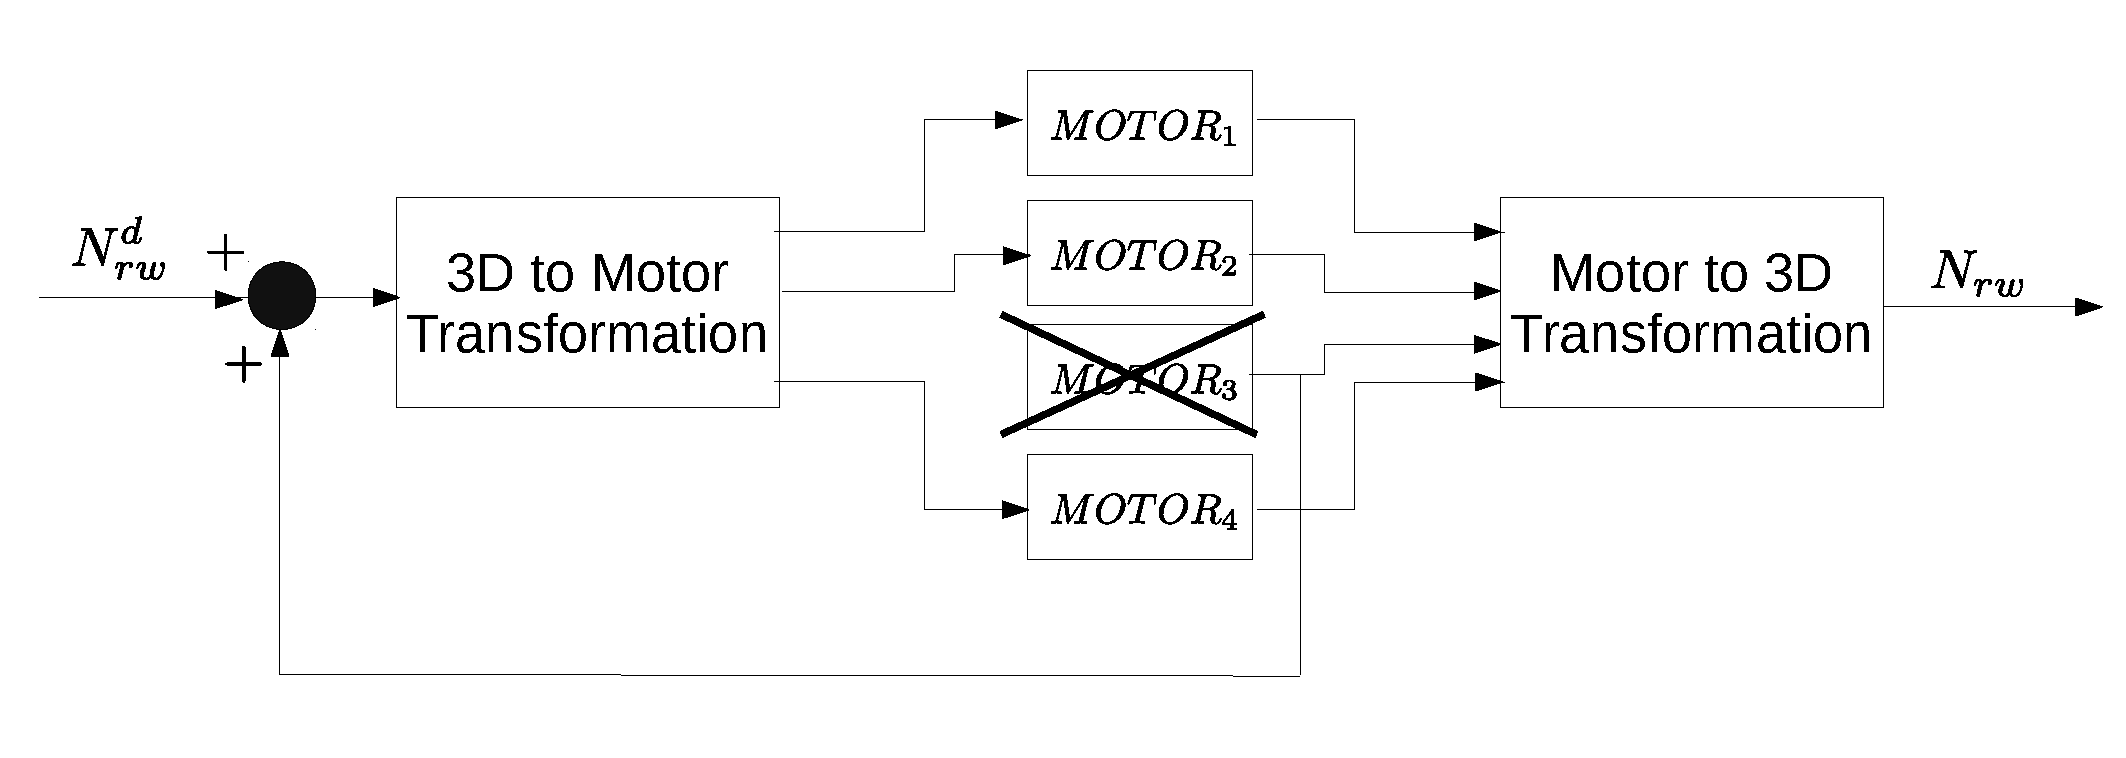
\includegraphics[width=120mm]{figures/residReconfigCompensation}
	\caption{Shutdown torque compensation in case of fault detected through residual.}
	\label{fig:resFaultCompensation}
\end{figure} 

%\begin{figure}
%	\centering
%	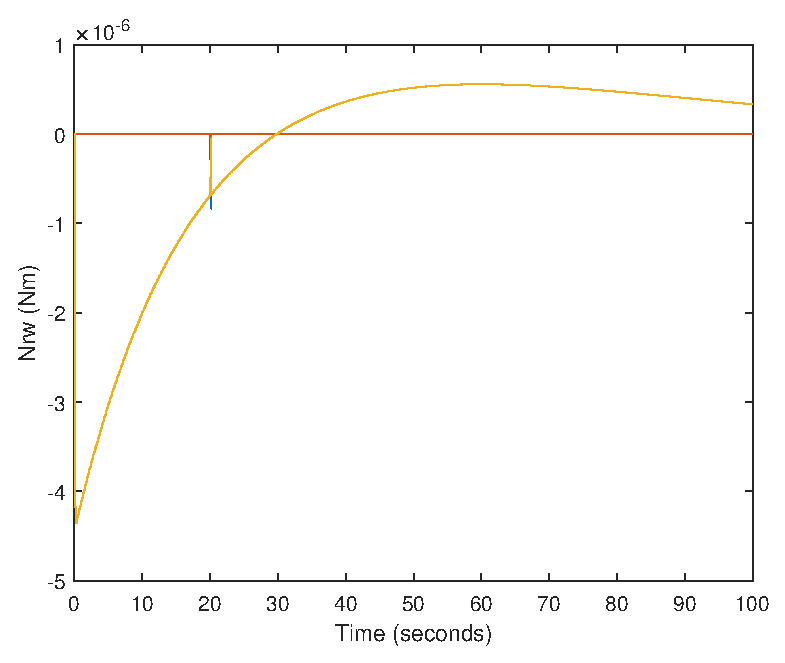
\includegraphics[width=120mm]{figures/3dTorque_resid_reconfig}
%	\caption{$N_rw$ with fault occuring at 20 seconds}
%\end{figure} 
%
%\begin{figure}
%	\centering
%	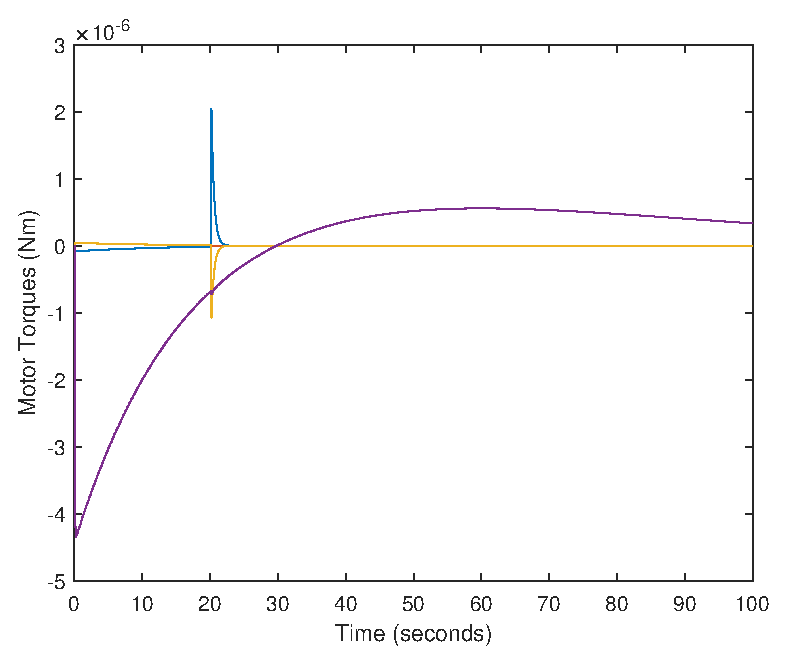
\includegraphics[width=120mm]{figures/torque_reconfig}
%	\caption{$N_M$ with fault occuring at 20 seconds}
%\end{figure} 
%
%\begin{figure}
%	\centering
%	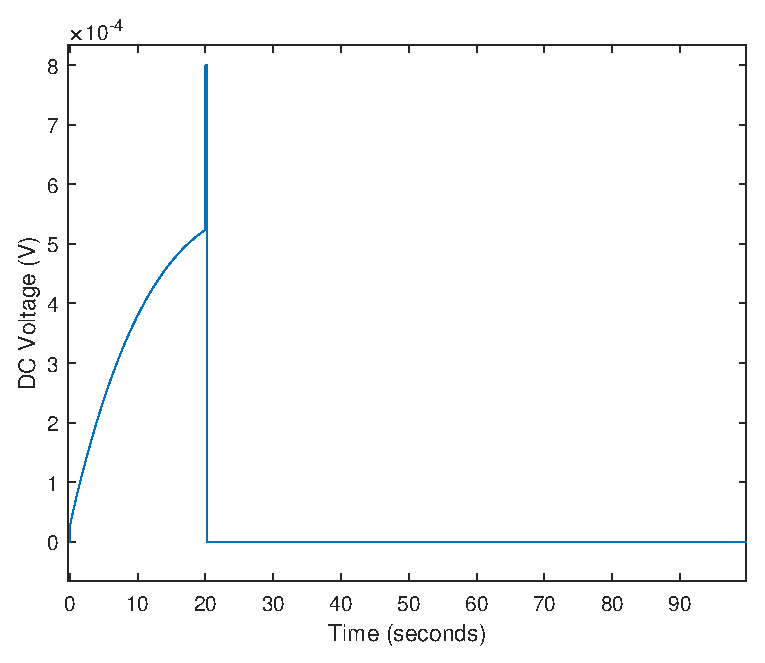
\includegraphics[width=120mm]{figures/voltage_reconfig}
%	\caption{Voltage control signal with fault occuring at 0 seconds}
%\end{figure} 
%
%
%\begin{figure}
%	\centering
%	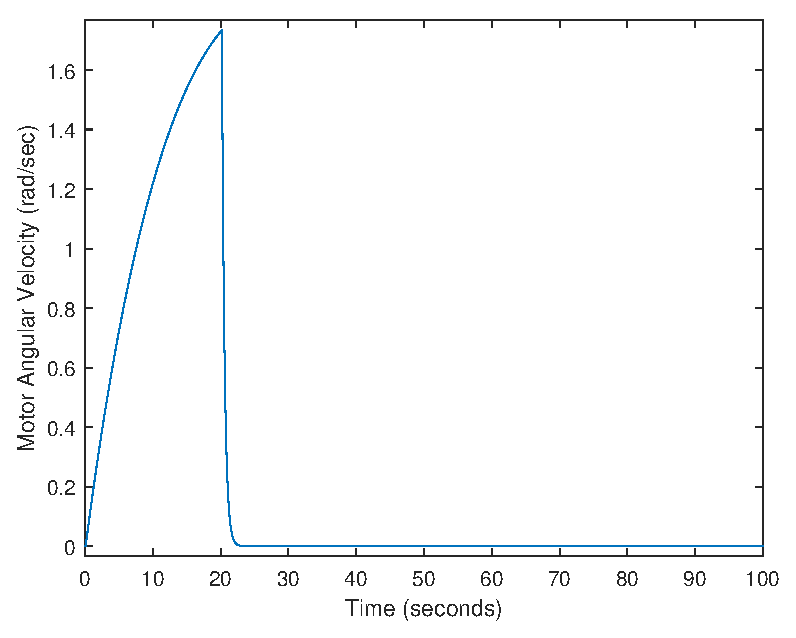
\includegraphics[width=120mm]{figures/omega_reconfig}
%	\caption{$\omega_{M,i}$ with fault occuring at 20 seconds}
%\end{figure} 
%
%
%\begin{figure}
%	\centering
%	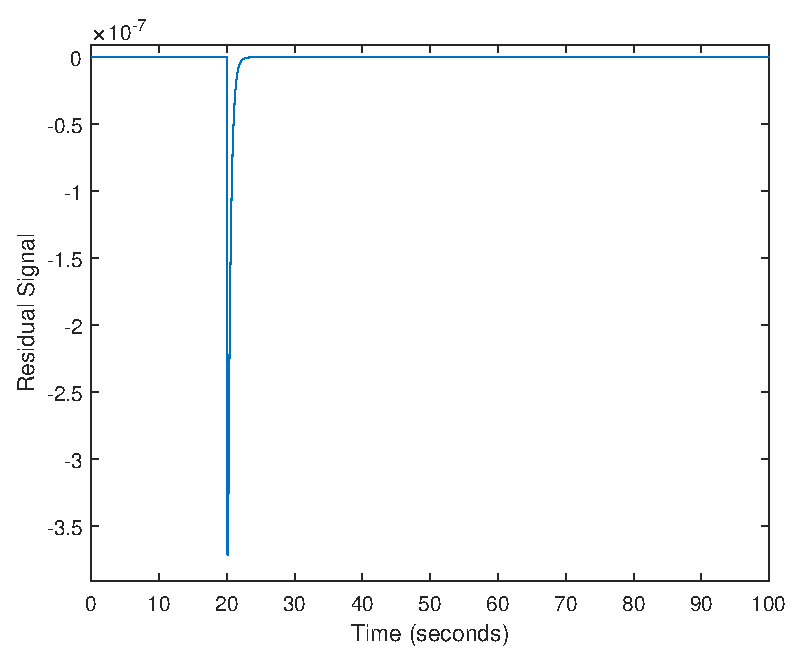
\includegraphics[width=120mm]{figures/residual_reconfig}
%	\caption{Residual signal with fault occuring at 20 seconds}
%\end{figure} 

\begin{figure}[H]
	\centering
	\begin{subfigure}{.5\textwidth}
	\centering
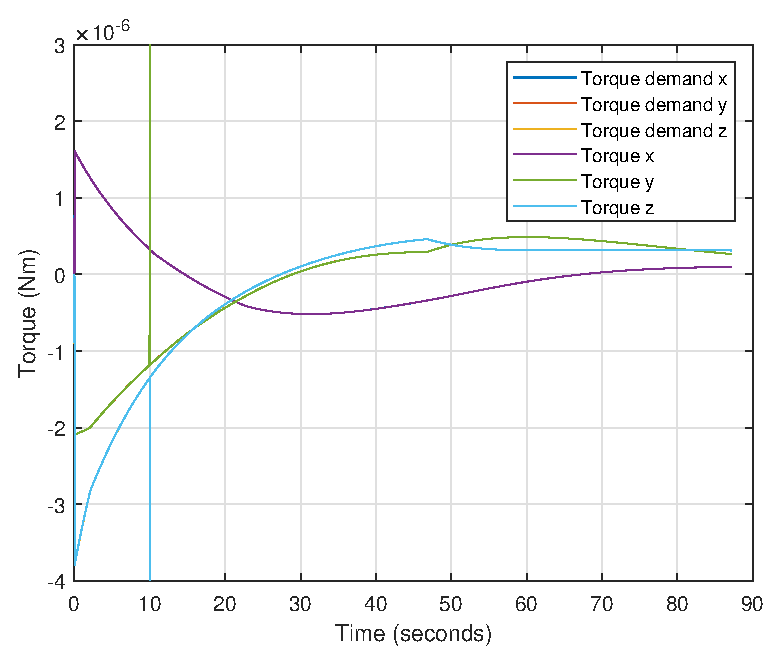
\includegraphics[width=70mm]{figures/smooth3dtorque}
\caption{}
	\label{fig:resreconfig_nrw}
	\end{subfigure}%
	\begin{subfigure}{.5\textwidth}
	\centering
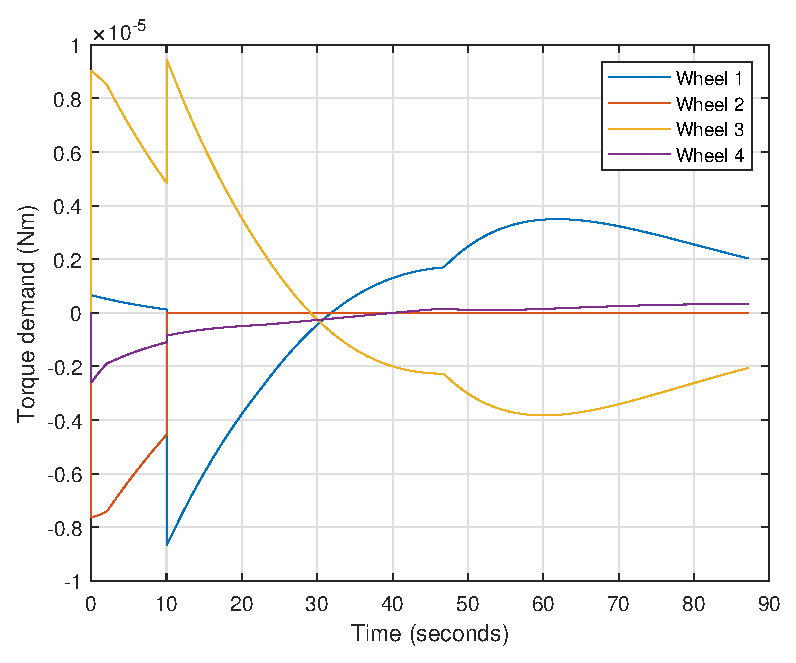
\includegraphics[width=70mm]{figures/smooth_motor_torque}
\caption{}
\label{fig:resreconfig_nm}
	\end{subfigure}
	\caption{Figure \ref{fig:resreconfig_nrw}: $N_{rw}$ with fault occuring at 10 seconds. Figure \ref{fig:resreconfig_nm}: $N_M$ with fault occuring at 10 seconds.}
	\label{fig:resreconfig}
\end{figure}

%\begin{figure}
%	\centering
%	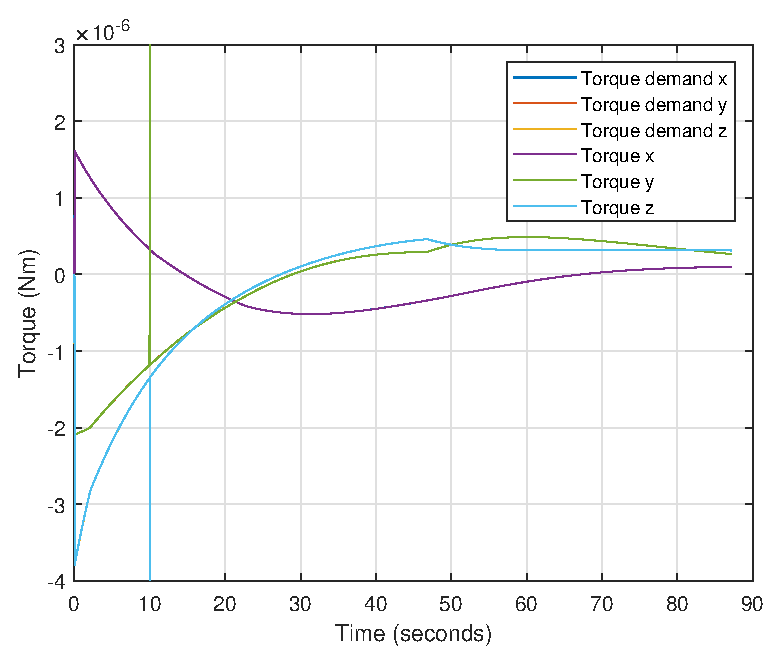
\includegraphics[width=120mm]{figures/smooth3dtorque}
%	\caption{$N_{rwn$ with fault occuring at 10 seconds}
%	\label{fig:resreconfig_nrw}
%\end{figure} 
%
%\begin{figure}
%	\centering
%	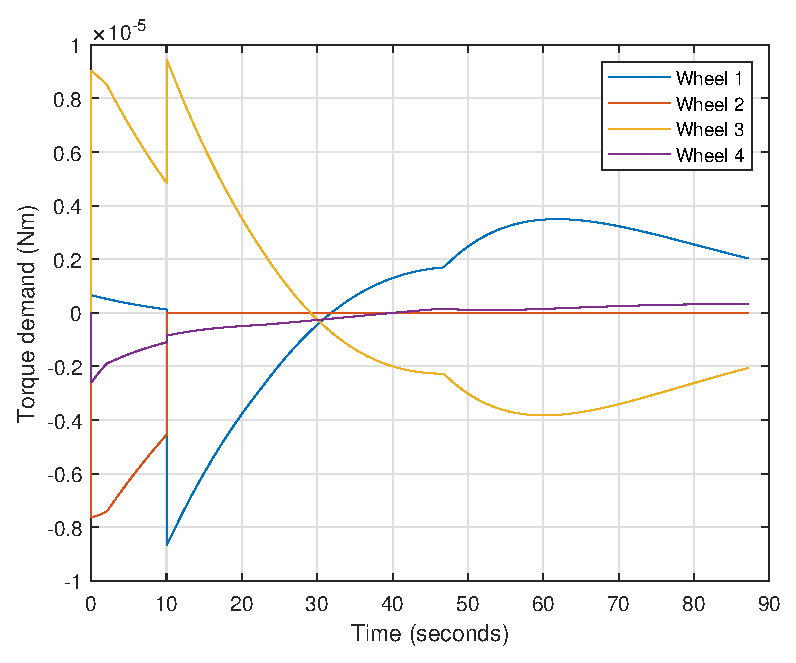
\includegraphics[width=120mm]{figures/smooth_motor_torque}
%	\caption{$N_M$ with fault occuring at 10 seconds}
%	\label{fig:resreconfig_nm}
%\end{figure} 

\begin{figure} [H]
\centering
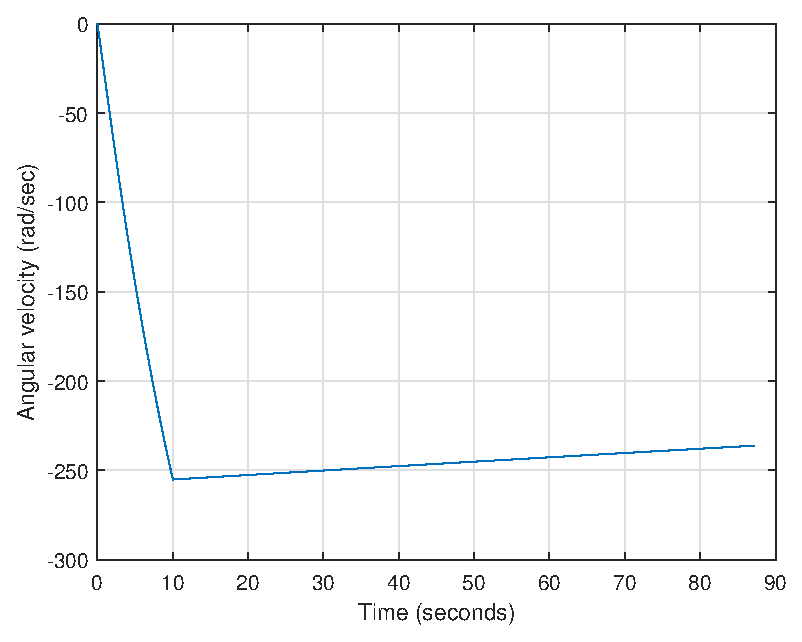
\includegraphics[width=70mm]{figures/smooth_omega_residual}
\caption{$\omega_{M,i}$ with fault occuring at 10 seconds}
\label{fig:resreconfig_ome}
\end{figure} 